\documentclass[conference]{IEEEtran}

% ----- Packages -----
\usepackage{graphicx}
\usepackage{booktabs}
\usepackage{url}
\usepackage{hyperref}
\usepackage{listings}
\usepackage{xcolor}
\usepackage{tikz}
\usepackage{amsmath}
\usepackage{multirow}
\usetikzlibrary{arrows.meta, positioning, shapes.geometric}

% ----- Hyperref -----
\hypersetup{
  colorlinks=true,
  linkcolor=black,
  urlcolor=blue,
  citecolor=black
}

% ----- Code listings -----
\lstset{
  basicstyle=\ttfamily\small,
  breaklines=true,
  frame=single,
  numbers=left,
  numberstyle=\tiny,
  xleftmargin=2em,
  framexleftmargin=1.5em,
  backgroundcolor=\color{gray!10}
}

% JSON listing style
\lstdefinelanguage{json}{
  basicstyle=\ttfamily\small,
  showstringspaces=false,
  breaklines=true,
  frame=single,
  backgroundcolor=\color{gray!10},
  literate=
   *{0}{{{\color{blue}0}}}{1}
    {1}{{{\color{blue}1}}}{1}
    {2}{{{\color{blue}2}}}{1}
    {3}{{{\color{blue}3}}}{1}
    {4}{{{\color{blue}4}}}{1}
    {5}{{{\color{blue}5}}}{1}
    {6}{{{\color{blue}6}}}{1}
    {7}{{{\color{blue}7}}}{1}
    {8}{{{\color{blue}8}}}{1}
    {9}{{{\color{blue}9}}}{1}
    {:}{{{\color{red}{:}}}}{1}
    {,}{{{\color{red}{,}}}}{1}
    {\{}{{{\color{black}{\{}}}}{1}
    {\}}{{{\color{black}{\}}}}}{1}
    {[}{{{\color{black}{[}}}}{1}
    {]}{{{\color{black}{]}}}}{1},
}

\title{Proposal: Construction.AI --- Knowledge-Graph + Agentic System for Material Takeoff, Cut Optimization, and Build Instructions}

\author{
\IEEEauthorblockN{Jason Cusati}
\IEEEauthorblockA{Construction.AI Project}
}

\begin{document}
\maketitle

% =============================================================================
% ABSTRACT
% =============================================================================
\begin{abstract}
This proposal describes a system that reads architectural plans and produces (1) an accurate bill of materials (BOM),
(2) optimized cut lists that reduce waste (e.g., selecting 12ft stock for an 11ft 6in cut instead of 16ft),
and (3) build instructions aligned with construction practices and applicable codes.
The system uses a Knowledge Graph (KG) to store structured information about components, materials, fasteners,
building rules, jurisdiction-specific regulations, and historical project outcomes.
A set of LLM-driven agents then queries the KG to infer assemblies, validate compliance, and generate outputs in
formats consumable by lumber yard and procurement systems.
\end{abstract}

% =============================================================================
% SECTIONS (modular files for easier editing)
% =============================================================================

% =============================================================================
% SECTION 1: MOTIVATION AND PROBLEM STATEMENT
% =============================================================================

\section{Motivation and Problem Statement}

Material takeoff---the process of extracting quantities from architectural plans---remains a critical bottleneck in construction estimation.
Estimators must infer assembly intent (e.g., header configurations, king stud packs, blocking patterns) from plan conventions and building codes.
Even with accurate BOMs, material waste remains high without stock-aware cut optimization.
Downstream stakeholders (framers, suppliers, project managers) require machine-readable outputs and detailed build instructions, not just raw quantities.

\subsection{Industry Challenges}

The construction industry faces persistent productivity gaps~\cite{mckinsey2017construction}:

\begin{itemize}
  \item \textbf{Time burden}: Professional estimators spend 50--80\% of their time on quantity takeoffs, limiting the number of bids they can process~\cite{rics2019takeoff}.
  A typical 2,000 sq.ft. residential frame takeoff requires 8--12 hours of manual work.

  \item \textbf{Error rates}: Manual measuring and counting leads to 10--15\% error rates in material estimates~\cite{deloitte2023outlook}, resulting in costly change orders, project delays, and strained supplier relationships.
  Common errors include miscounting studs for wall intersections, incorrect header sizing, and missing blocking requirements.

  \item \textbf{Inconsistency}: Two estimators working from the same plans often produce BOMs differing by 5--10\% in key materials like lumber and fasteners, undermining cost predictability.

  \item \textbf{Knowledge gaps}: Junior estimators lack deep knowledge of framing methodology and jurisdiction-specific code requirements (IRC~\cite{irc2021}, local amendments), leading to non-compliant or over-conservative designs.

  \item \textbf{Material waste}: Without cut optimization, lumber waste rates of 15--20\% are typical; optimized systems demonstrate waste reduction to under 5\%~\cite{manrique2007framex}, representing significant cost savings on large projects.
\end{itemize}

\subsection{Goals}

\textbf{Goal:} Create an end-to-end workflow that:
\begin{enumerate}
  \item[(a)] Interprets plans into \emph{component assemblies} (walls, headers, openings)
  \item[(b)] Selects \emph{real-world purchasable stock} (lengths, grades, treatments)
  \item[(c)] Computes \emph{cuts with waste minimization} using optimization algorithms
  \item[(d)] Exports data in \emph{supplier-friendly formats} (CSV, JSON, EDI)
  \item[(e)] Generates \emph{build instructions} with code compliance citations
\end{enumerate}

% =============================================================================
% SECTION 2A: RELATED WORK AND NOVELTY
% =============================================================================

\section{Related Work and Contributions}

\subsection{Existing Approaches}

Current construction takeoff solutions fall into three categories:

\textbf{Manual/Semi-Automated Tools.}
Traditional tools like PlanSwift~\cite{planswift2024} and Bluebeam require human operators to trace elements and apply counts.
While accurate, they scale poorly and depend on operator expertise.

\textbf{Rule-Based Estimation.}
Commercial systems (e.g., STACK~\cite{stack2024}) embed framing rules in code, limiting adaptability across jurisdictions and practices.
Rule updates require software modifications, and decisions lack auditability.

\textbf{AI-Powered Takeoff.}
Recent AI tools (e.g., Togal.AI~\cite{togalai2024}) use computer vision to detect areas and count symbols~\cite{pizarro2022floorplan_survey, jamieson2025symbol_detection},
but typically output quantities without assembly reasoning, cut optimization, or code compliance verification.

\subsection{Limitations of Prior Work}

\begin{enumerate}
  \item \textbf{Embedded knowledge}: Rules and practices are hard-coded, not inspectable or versionable
  \item \textbf{Missing provenance}: BOM line items cannot be traced to plan facts and applied rules
  \item \textbf{No optimization}: Stock selection and cutting are left to downstream processes
  \item \textbf{Limited compliance}: Code citations require manual verification
  \item \textbf{No learning}: Systems do not improve from project outcomes
\end{enumerate}

\subsection{Key Contributions}

This proposal presents the following novel contributions:

\begin{enumerate}
  \item \textbf{KG-Centered Architecture}: A knowledge graph backbone that externalizes construction rules, material catalogs, and historical precedents---enabling inspection, versioning, and auditing~\cite{pan2024unifying_kg_llm}.

  \item \textbf{Provenance-First Design}: Every BOM line item links to (a) plan facts, (b) applied inference rules, and (c) code references, supporting explainability and regulatory compliance.

  \item \textbf{Multi-Agent Reasoning}: Specialized agents for extraction QA, component inference, compliance checking, and instruction generation~\cite{li2025agentic_survey, zhang2025tool_learning}, with clear separation from deterministic optimization.

  \item \textbf{Integrated Cut Optimization}: Stock selection and cutting as a first-class concern, using ILP solvers~\cite{ortools2024} with kerf handling and multi-stock support~\cite{gilmore1961cutting}.

  \item \textbf{Continuous Improvement Loop}: Human corrections and project outcomes feed back into the KG as new precedents, enabling system-wide learning.
\end{enumerate}

\subsection{Differentiation Summary}

Table~\ref{tab:differentiation} compares our approach to existing solutions.

\begin{table}[ht]
\centering
\caption{Comparison with Existing Approaches}
\label{tab:differentiation}
\begin{tabular}{lcc}
\toprule
\textbf{Capability} & \textbf{Existing} & \textbf{Ours} \\
\midrule
Knowledge storage & Code-embedded & KG-externalized \\
Rule versioning & Manual updates & Temporal validity \\
Provenance & None/limited & Full chain \\
Cut optimization & Separate/none & Integrated \\
Compliance & Manual check & Auto w/ citations \\
Learning & Static & Continuous \\
\bottomrule
\end{tabular}
\end{table}

% =============================================================================
% SECTION 2: SYSTEM ARCHITECTURE OVERVIEW
% =============================================================================

\section{System Architecture Overview}
\label{sec:arch}

Figure~\ref{fig:arch} summarizes the proposed architecture.
The design follows three architectural patterns common in modern AI systems~\cite{lewis2020rag}:

\textbf{(1) Retrieval-Augmented Generation (RAG)}---agents retrieve relevant facts from the KG before generating outputs, grounding decisions in structured knowledge rather than parametric memory alone.

\textbf{(2) Tool-Augmented Agents}---LLM agents invoke deterministic tools (optimizer, exporter) for tasks requiring provable correctness~\cite{schick2023toolformer}.

\textbf{(3) Blackboard Architecture}---the KG serves as a shared workspace where specialized agents read inputs, write inferences, and coordinate asynchronously.

The core design principle is that the system is \emph{KG-centered}: extracted plan facts and inferred construction intent are continuously grounded against a structured graph of rules, components, and historical builds.

\begin{figure}[ht]
\centering
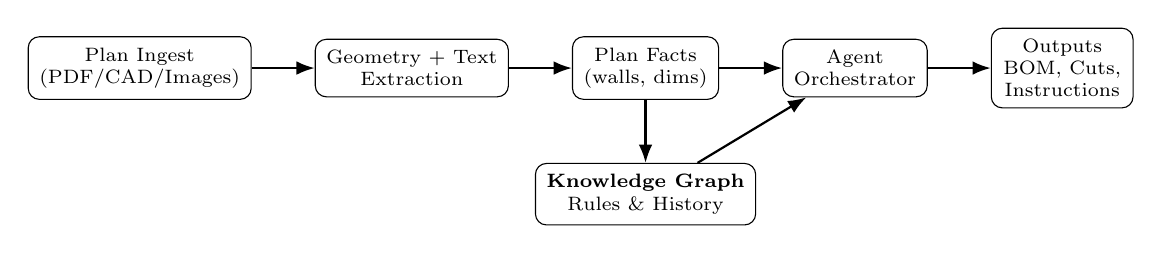
\begin{tikzpicture}[
  node distance=6mm and 8mm,
  box/.style={draw, rounded corners, align=center, inner sep=4pt, font=\scriptsize, minimum width=18mm},
  arrow/.style={-Latex, thick}
]
\node[box] (ingest) {Plan Ingest\\(PDF/CAD/Images)};
\node[box, right=of ingest] (extract) {Geometry + Text\\Extraction};
\node[box, right=of extract] (facts) {Plan Facts\\(walls, dims)};
\node[box, below=8mm of facts] (kg) {\textbf{Knowledge Graph}\\Rules \& History};
\node[box, right=of facts] (agents) {Agent\\Orchestrator};
\node[box, right=of agents] (outputs) {Outputs\\BOM, Cuts,\\Instructions};

\draw[arrow] (ingest) -- (extract);
\draw[arrow] (extract) -- (facts);
\draw[arrow] (facts) -- (agents);
\draw[arrow] (kg) -- (agents);
\draw[arrow] (facts) -- (kg);
\draw[arrow] (agents) -- (outputs);
\end{tikzpicture}
\caption{KG-centered architecture: plan facts are extracted, normalized, stored with provenance, and used by agents to generate compliant, optimized outputs.}
\label{fig:arch}
\end{figure}

\subsection{Key Modules}

\textbf{(1) Plan Ingest + Extraction.}
Convert drawings into machine-usable primitives:
vector geometry (lines, polylines), detected room/wall boundaries, and text tokens (dimensions, callouts, schedules)~\cite{pizarro2022floorplan_survey}.
The current implementation supports PDF (via PyMuPDF~\cite{pymupdf2024}), DXF (via ezdxf~\cite{ezdxf2024}), and DWG (via LibreDWG conversion).
For raster images, YOLOv8 object detection~\cite{jocher2023yolov8} and EasyOCR~\cite{easyocr2024} provide robust extraction.

\textbf{(2) Plan Facts Model.}
Normalize extraction into a consistent intermediate representation:
\emph{WallSegments}, \emph{Openings}, \emph{Headers}, \emph{Notes}, \emph{Schedules}, and \emph{Constraints}
with explicit provenance back to the sheet, region, and confidence score.

\textbf{(3) Knowledge Graph.}
Store rules, materials, codes, and historical knowledge (Section~\ref{sec:kg}).

\textbf{(4) Agent Orchestrator.}
A multi-agent workflow that queries the KG, performs reasoning and validation,
and calls deterministic optimization routines for cutting and procurement.

\textbf{(5) Export + Integration.}
Produce both human-usable artifacts (PDF/HTML summaries, build steps)
and machine-readable exports (CSV/JSON/EDI-style mappings) suitable for lumber yard systems.

\subsection{Data Flow}

The system operates in five sequential phases:

\textbf{Phase 1: Extraction.}
Plan documents are parsed into vector geometry, raster images, and text.
YOLOv8 detects symbols; PyMuPDF extracts text and vectors from PDFs; ezdxf handles CAD formats.
Output: raw geometry primitives and text tokens with bounding boxes.

\textbf{Phase 2: Normalization.}
Raw extraction is normalized into \texttt{PlanFact} nodes in the KG, each with source provenance (sheet, region, confidence).
Cross-validation checks dimension consistency and flags ambiguities.

\textbf{Phase 3: Inference.}
Agents query the KG for plan facts and rules, then write inferred assemblies (\texttt{AssemblyIntent}, \texttt{Component}) back to the KG.
Each inference links to triggering facts and applied rules.

\textbf{Phase 4: Optimization.}
The Procurement Agent selects stock items and invokes the cut-stock optimizer (ILP solver) for waste minimization.
Results are written as \texttt{CutPiece} nodes linked to source components.

\textbf{Phase 5: Export.}
Final outputs (BOM, cut lists, instructions) are generated by querying the KG and formatting results.
Every output line item carries provenance links back through phases 4→3→2→1.

% =============================================================================
% SECTION 3: KNOWLEDGE GRAPH DESIGN
% =============================================================================

\section{Knowledge Graph Design}
\label{sec:kg}

The knowledge graph (KG) serves as the backbone for \emph{grounded, repeatable decisions}~\cite{hogan2021kg_survey, zheng2022kg_construction}.
Unlike rule-based systems that embed logic in code, the KG externalizes knowledge so it can be inspected, updated, and audited independently of the reasoning engine.

\subsection{Theoretical Foundation}

Knowledge graphs represent information as a labeled, directed multi-graph $G = (V, E, L)$ where vertices $V$ represent entities, edges $E \subseteq V \times V$ represent relationships, and $L$ provides type labels~\cite{hogan2021kg_survey}.
This formalism supports:

\begin{itemize}
  \item \textbf{Explicit semantics}: Relationships are first-class citizens with types and properties
  \item \textbf{Schema flexibility}: New entity and relationship types can be added without migration
  \item \textbf{Path queries}: Multi-hop reasoning (e.g., ``which code rules constrain this header?'')
  \item \textbf{Provenance tracking}: Every fact can carry source attribution
\end{itemize}

Pan et al.~\cite{pan2024unifying_kg_llm} identify three paradigms for KG-LLM integration: KG-enhanced LLMs, LLM-augmented KGs, and synergized systems.
Our architecture follows the synergized approach, where agents query the KG for grounded facts and update it with validated inferences.

\subsection{Why Not Alternatives?}

We considered three alternative knowledge representations:

\textbf{Rule engines} (e.g., Drools, CLIPS) excel at forward/backward chaining but embed rules in code or DSL files.
Rules are difficult to inspect, version, and explain to end users.
When rules conflict, debugging requires developer intervention.

\textbf{Ontologies} (e.g., OWL/RDF) provide formal semantics and reasoning via description logics~\cite{pauwels2017kg_ifc}.
However, OWL reasoners struggle with scale, closed-world assumptions conflict with construction's open-world nature, and the formalism is inaccessible to domain experts.

\textbf{Relational databases} handle structured data well but require JOIN-heavy queries for relationship traversal.
A query like ``find all components constrained by IRC R602.3'' requires multiple joins across normalized tables; in a graph, it is a single-hop traversal.

The KG approach balances expressiveness, scalability, and maintainability for construction domain knowledge.

\subsection{Knowledge Categories}

The KG organizes construction knowledge into six categories:

\begin{itemize}
  \item \textbf{Component definitions}: studs, headers, plates, cripples, blocking, sheathing---with parameterized assemblies
  \item \textbf{Material catalog}: dimensions, grades, treatments, SKUs, stock lengths, pricing, lead times
  \item \textbf{Fasteners and connectors}: nails, screws, straps, hangers, anchors---with application rules and schedules
  \item \textbf{Building rules}: framing conventions, span tables, loading assumptions, nailing patterns
  \item \textbf{Codes and regulations}: jurisdiction, version, section citations, applicability conditions
  \item \textbf{Historical precedents}: past project decisions, substitutions, waste rates, outcome feedback
\end{itemize}

\subsection{Core Entities and Relationships}

Table~\ref{tab:kg_entities} summarizes the core entity types, and Table~\ref{tab:kg_relationships} shows key relationships.

\begin{table}[ht]
\centering
\caption{Core KG Entity Types}
\label{tab:kg_entities}
\begin{tabular}{ll}
\toprule
\textbf{Entity Type} & \textbf{Description} \\
\midrule
Project & Building project with metadata \\
PlanSheet & Individual plan page with scale \\
PlanFact & Extracted fact with confidence \\
AssemblyIntent & Inferred assembly (e.g., header) \\
Component & Physical component instance \\
StockItem & Purchasable material \\
CutPiece & Result of cutting operation \\
CodeRule & Building code requirement \\
FastenerRule & Fastening specification \\
Supplier & Material supplier \\
\bottomrule
\end{tabular}
\end{table}

\begin{table}[ht]
\centering
\caption{Core KG Relationship Types}
\label{tab:kg_relationships}
\begin{tabular}{lll}
\toprule
\textbf{Relationship} & \textbf{From} & \textbf{To} \\
\midrule
hasSheet & Project & PlanSheet \\
mentions & PlanSheet & PlanFact \\
instantiates & PlanFact & AssemblyIntent \\
composedOf & AssemblyIntent & Component \\
builtFrom & Component & StockItem \\
cutInto & StockItem & CutPiece \\
constrainedBy & Component & CodeRule \\
requiresFastener & Component & FastenerRule \\
suppliedBy & StockItem & Supplier \\
\bottomrule
\end{tabular}
\end{table}

\subsection{Example Query: Provenance Chain}

The following Cypher query retrieves the full provenance chain for a BOM line item, demonstrating the KG's traceability:

\begin{lstlisting}[language=json, basicstyle=\ttfamily\scriptsize]
MATCH (bom:BOMItem {id: $itemId})
      -[:derivedFrom]->(cut:CutPiece)
      -[:cutFrom]->(stock:StockItem)
      <-[:builtFrom]-(comp:Component)
      <-[:composedOf]-(asm:AssemblyIntent)
      <-[:instantiates]-(fact:PlanFact)
      -[:extractedFrom]->(sheet:PlanSheet)
OPTIONAL MATCH (comp)-[:constrainedBy]->(code:CodeRule)
RETURN bom, cut, stock, comp, asm, fact,
       sheet, collect(code) as codeRules
\end{lstlisting}

This single query traverses the entire chain from BOM output back to plan source, collecting all applicable code rules---a query that would require 6+ JOINs in a relational model.

\subsection{Versioning and Provenance}

Construction knowledge evolves: codes are updated, suppliers change SKUs, practices differ by region.
The KG supports this through:

\begin{itemize}
  \item \textbf{Temporal validity}: Effective dates and regions on CodeRule and MaterialSpec nodes
  \item \textbf{Source provenance}: Document reference, section number, URL/file hash on every fact
  \item \textbf{Decision audit}: Agent decisions are logged with reasoning traces linked to KG facts
\end{itemize}

Every generated BOM line item links back to: (1) which plan facts triggered it, (2) which inference rules were applied, and (3) which code references constrained it.

\subsection{Technology Choice: Neo4j}

We select Neo4j as the graph database platform based on:

\begin{itemize}
  \item \textbf{Native graph storage}: Index-free adjacency enables O(1) relationship traversal regardless of graph size~\cite{neo4j2023construction}
  \item \textbf{Cypher query language}: Declarative pattern matching for complex multi-hop queries
  \item \textbf{Vector index support}: Native vector similarity search enables GraphRAG patterns~\cite{edge2024graphrag, lewis2020rag}
  \item \textbf{APOC procedures}: Graph algorithms (centrality, community detection) for analytics
  \item \textbf{Python ecosystem}: Async driver compatible with FastAPI; LangChain integration available
\end{itemize}

Alternative graph databases (Amazon Neptune, TigerGraph) were considered but Neo4j's developer tooling, community support, and vector search capabilities made it the pragmatic choice for this domain.

% =============================================================================
% SECTION 4: DATA SOURCES, CURATION, AND GROUND TRUTH
% =============================================================================

\section{Data: Sources, Curation, and Ground Truth}

\subsection{Input Types}

\begin{itemize}
  \item \textbf{Vector CAD}: DXF/DWG files with layer-organized geometry
  \item \textbf{PDF Plans}: Both vector PDFs and scanned raster images
  \item \textbf{Schedules}: Door/window schedules, material legends
  \item \textbf{Specifications}: Project specs with material requirements
  \item \textbf{As-built data}: Jobsite photos, marked-up drawings
\end{itemize}

\subsection{Ground Truth Strategy}

\begin{enumerate}
  \item Start with completed projects where final lumber orders and framing decisions are known
  \item Align plan-derived assemblies with actual purchase orders and observed waste
  \item Create manually labeled subset (50--100 residential sheets) verified by estimators
  \item Capture human overrides as new precedents in the KG
\end{enumerate}

\subsection{Curation Loop}

When the system encounters ambiguous cases (e.g., missing header callout, unclear wall type):
\begin{enumerate}
  \item Propose options with confidence scores and citations
  \item Record human selections back into the KG as new precedent
  \item Track which rules produced correct vs. incorrect inferences
  \item Continuously improve confidence calibration
\end{enumerate}

% =============================================================================
% SECTION 5: AGENTIC WORKFLOW
% =============================================================================

\section{Agentic Workflow}

Agents are responsible for \emph{turning facts into decisions}, while deterministic tools handle optimization and exporting~\cite{wang2024agents_survey, xi2023agents_rise, li2025agentic_survey}.
Recent surveys on tool-augmented LLMs~\cite{zhang2025tool_learning} demonstrate the effectiveness of separating reasoning from tool invocation.
This separation ensures that reasoning is auditable and optimization is provably correct.

\subsection{Agent Architecture}

\begin{figure}[ht]
\centering
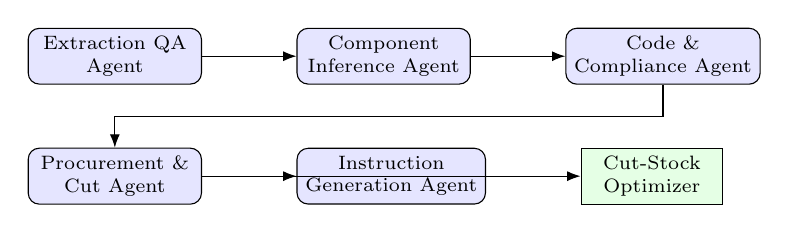
\begin{tikzpicture}[
  node distance=5mm and 12mm,
  agent/.style={draw, rounded corners, align=center, inner sep=3pt, font=\scriptsize, fill=blue!10, minimum width=22mm},
  tool/.style={draw, align=center, inner sep=3pt, font=\scriptsize, fill=green!10, minimum width=18mm},
  arrow/.style={-Latex}
]
\node[agent] (qa) {Extraction QA\\Agent};
\node[agent, right=of qa] (infer) {Component\\Inference Agent};
\node[agent, right=of infer] (code) {Code \&\\Compliance Agent};
\node[agent, below=8mm of qa] (procure) {Procurement \&\\Cut Agent};
\node[agent, right=of procure] (instruct) {Instruction\\Generation Agent};
\node[tool, right=of instruct] (optimizer) {Cut-Stock\\Optimizer};

\draw[arrow] (qa) -- (infer);
\draw[arrow] (infer) -- (code);
\draw[arrow] (code.south) -- ++(0,-4mm) -| (procure.north);
\draw[arrow] (procure) -- (instruct);
\draw[arrow] (procure) -- (optimizer);
\end{tikzpicture}
\caption{Agent workflow: specialized agents handle extraction QA, component inference, compliance checking, procurement, and instruction generation.}
\label{fig:agents}
\end{figure}

\subsection{Extraction QA Agent}

Validates extracted geometry/text, flags low-confidence dimensions, and requests targeted reprocessing:
\begin{itemize}
  \item Dimension consistency checks (wall lengths match floor plan scale)
  \item Missing element detection (walls without openings noted)
  \item OCR confidence thresholds (request higher DPI on region if below threshold)
\end{itemize}

\subsection{Component Inference Agent}

Maps plan facts to assemblies using KG rules:
\begin{itemize}
  \item Wall type $\rightarrow$ stud size/spacing, plates, sheathing type
  \item Opening size $\rightarrow$ header assembly, jack/king studs, cripples
  \item Notes/schedules $\rightarrow$ material upgrades, fastener patterns
  \item Bearing vs. non-bearing $\rightarrow$ header sizing, stud requirements
\end{itemize}

\subsection{Code \& Compliance Agent}

Checks assemblies against code rules stored in the KG (jurisdiction/version)~\cite{zhang2023kg_codes, beach2020irc_automation}:
\begin{itemize}
  \item Validates header sizing for span/load per IRC~\cite{irc2021}
  \item Checks stud spacing for load-bearing walls
  \item Verifies fastener patterns (nailing schedules)
  \item Produces ``compliant'' or ``requires review'' with citations
\end{itemize}

\subsection{Procurement \& Cut Optimization Agent}

Selects purchasable stock and calls the cut-stock optimizer:
\begin{itemize}
  \item Allowed stock lengths (8/10/12/14/16/20 ft, LVL lengths, panel sizes)
  \item Kerf allowance (0.125'') and defect waste factor
  \item Bundling rules (keep identical cuts together for crew efficiency)
  \item Substitution rules (use 12ft if it avoids waste; prefer in-stock SKUs)
\end{itemize}

\subsection{Instruction Generation Agent}

Generates build instructions that reference assemblies, cut pieces, and fastening rules:
\begin{itemize}
  \item Organized by wall line, room, or framing phase
  \item ``What to build'' with component references
  \item ``How to fasten'' with fastener specs and patterns
  \item ``Inspection callouts'' with code citations
\end{itemize}

% =============================================================================
% SECTION 6: KEY TECHNOLOGIES
% =============================================================================

\section{Key Technologies}

\subsection{Parsing Stack}

\begin{table}[ht]
\centering
\caption{Parsing Technologies}
\label{tab:parsing}
\begin{tabular}{ll}
\toprule
\textbf{Format} & \textbf{Technology} \\
\midrule
PDF (vector) & PyMuPDF (fitz) \\
PDF (raster) & pdf2image + OpenCV \\
DXF & ezdxf \\
DWG & LibreDWG $\rightarrow$ DXF \\
OCR & EasyOCR, Tesseract \\
Object Detection & YOLOv8~\cite{rezvanifar2020yolo_symbols, kalervo2019cubicasa5k} \\
Scale Detection & Google Gemini Vision API \\
\bottomrule
\end{tabular}
\end{table}

\subsection{Cut Optimization}

The cutting stock problem is NP-hard but well-studied~\cite{gilmore1961cutting, wascher2007csp_survey}. We employ:
\begin{itemize}
  \item \textbf{Heuristics}: First-Fit Decreasing (FFD) for fast, decent solutions
  \item \textbf{Exact methods}: Integer Linear Programming via OR-Tools~\cite{ortools2024} or PuLP
  \item \textbf{Kerf handling}: Each cut consumes blade width (0.125''); $n$ pieces require $(n-1) \times \text{kerf}$~\cite{cui2017lumber_optimization}
  \item \textbf{Multi-stock}: Optimize across available stock lengths simultaneously
\end{itemize}

Objective function:
\begin{equation}
\min \sum_{s \in S} c_s \cdot x_s + \lambda \cdot \text{waste}
\end{equation}
where $x_s$ is the count of stock length $s$, $c_s$ is cost, and $\lambda$ weights waste penalty.

\subsection{Knowledge Graph Stack}

Recent advances in LLM-KG integration~\cite{zhu2024llm_kg_construction} inform our technology choices:
\begin{itemize}
  \item \textbf{Graph Database}: Neo4j Community/Enterprise
  \item \textbf{Query Language}: Cypher
  \item \textbf{Python Driver}: neo4j (async compatible)
  \item \textbf{Embeddings}: OpenAI/Anthropic for semantic search
  \item \textbf{Vector Index}: Neo4j vector index with GraphRAG patterns~\cite{edge2024graphrag}
\end{itemize}

\subsection{Agent Framework}

\begin{itemize}
  \item \textbf{LLM}: Claude~\cite{anthropic2024claude} or GPT-4~\cite{openai2024gpt4}
  \item \textbf{Orchestration}: LangChain~\cite{chase2022langchain} or custom agent loop following ReAct patterns~\cite{yao2023react}
  \item \textbf{Tool Calling}: Structured function calls to KG, optimizer, exporters~\cite{schick2023toolformer}
  \item \textbf{Memory}: Conversation context + KG query results
\end{itemize}

% =============================================================================
% SECTION 7: OUTPUTS AND SUPPLIER INTEGRATION
% =============================================================================

\section{Outputs and Supplier Integration}

\subsection{Output Types}

\begin{enumerate}
  \item \textbf{Bill of Materials (BOM)}: Multi-level hierarchy (project $\rightarrow$ wall $\rightarrow$ assembly $\rightarrow$ stock items)
  \item \textbf{Cut Lists}: Grouped by stock length and material type, with labeled cut pieces
  \item \textbf{Fastener List}: Nails, screws, anchors, straps, hangers with quantities
  \item \textbf{Build Instructions}: Step-by-step with plan sheet references and code notes
  \item \textbf{Compliance Report}: Code citations, validation status, items requiring review
\end{enumerate}

\subsection{Export Formats}

\begin{itemize}
  \item \textbf{CSV}: Lumber yard import (SKU, qty, length, treatment, notes)
  \item \textbf{JSON}: Structured assemblies + cuts + provenance
  \item \textbf{PDF/HTML}: Human-readable reports with diagrams
  \item \textbf{EDI}: Optional mapping layer for specific suppliers
\end{itemize}

\subsection{Sample JSON Structure}

\begin{lstlisting}[language=json]
{
  "project": "9557 Barnes Road",
  "assemblies": [{
    "type": "header_assembly",
    "opening": "Front Door",
    "components": [{
      "type": "header",
      "spec": "(2) 2x10",
      "length_in": 42,
      "stock_length": 144,
      "waste_in": 102
    }],
    "fasteners": [{
      "type": "16d common",
      "qty": 24,
      "pattern": "3\" O.C."
    }],
    "code_ref": "IRC R602.7"
  }]
}
\end{lstlisting}

% =============================================================================
% SECTION 8: PHASED DEVELOPMENT PLAN
% =============================================================================

\section{Phased Development Plan}

\subsection{Phase 1: KG Foundation + Enhanced Takeoff (4--6 weeks)}

\begin{itemize}
  \item Define initial ontology in Neo4j
  \item Migrate existing lumber calculations to KG-backed rules
  \item Load baseline component definitions and framing rules
  \item Parse 2--3 plan sets with provenance tracking
  \item Generate BOM with rule citations
\end{itemize}

\subsection{Phase 2: Assembly Reasoning + Cut Optimization (6--10 weeks)}

\begin{itemize}
  \item Expand component library (headers, stud packs, plates, sheathing)
  \item Implement Component Inference Agent with KG queries
  \item Integrate OR-Tools cut-stock optimizer
  \item Produce supplier-ready cut list exports
  \item Validate against ground truth projects
\end{itemize}

\subsection{Phase 3: Code/Regulation Layer (6--10 weeks)}

\begin{itemize}
  \item Model IRC/IBC code rules with jurisdiction and version
  \item Implement Code \& Compliance Agent
  \item Add compliance citations to outputs
  \item Build code rule editor for jurisdiction customization
\end{itemize}

\subsection{Phase 4: Feedback Loop + Learning (Ongoing)}

\begin{itemize}
  \item Capture user overrides and corrections
  \item Store outcomes (actual waste, substitutions made)
  \item Continuously improve confidence calibration
  \item Expand KG with new precedents
\end{itemize}

% =============================================================================
% SECTION 9: CURRENT IMPLEMENTATION STATUS
% =============================================================================

\section{Current Implementation Status}

Building on established approaches for BIM-based quantity extraction~\cite{eastman2018bim, eldiraby2017bim_quantities}, the following components are already implemented in the construction-ai codebase:

\begin{table}[ht]
\centering
\caption{Implementation Status}
\label{tab:status}
\begin{tabular}{lcc}
\toprule
\textbf{Component} & \textbf{Status} & \textbf{Phase} \\
\midrule
DXF/DWG Parsing & Complete & 1 \\
PDF Parsing & Complete & 1 \\
Wall Extraction & Complete & 1 \\
Stud/Plate Calculation & Complete & 1 \\
YOLOv8 Object Detection & Partial & 2 \\
Gemini Scale Detection & Complete & 1 \\
Web Interface (React) & Complete & 1 \\
PostgreSQL Database & Complete & 1 \\
Docker Infrastructure & Complete & 1 \\
\midrule
Neo4j Knowledge Graph & \textbf{New} & 1--2 \\
Agent Orchestration & \textbf{New} & 2 \\
Cut Optimization & \textbf{New} & 2 \\
Code Compliance & \textbf{New} & 3 \\
Build Instructions & \textbf{New} & 3 \\
\bottomrule
\end{tabular}
\end{table}

% =============================================================================
% SECTION 10: SCALABILITY AND FUTURE ENHANCEMENTS
% =============================================================================

\section{Scalability and Future Enhancements}

\subsection{Performance Targets}

The system targets production-grade performance for concurrent multi-user scenarios:

\begin{table}[ht]
\centering
\caption{Performance Targets}
\label{tab:perf_targets}
\begin{tabular}{lc}
\toprule
\textbf{Metric} & \textbf{Target} \\
\midrule
Plan processing time & <2 min (20-sheet residential) \\
Concurrent users & 100+ simultaneous \\
KG query latency & <100ms (95th percentile) \\
Cut optimization & <30s (500-piece list) \\
BOM generation & <10s per project \\
System availability & 99.5\% uptime \\
\bottomrule
\end{tabular}
\end{table}

\subsection{Architecture for Scale}

\textbf{Database Layer:}
\begin{itemize}
  \item Neo4j cluster (3+ nodes) with read replicas for query load distribution
  \item Sharding strategy: Tenant-isolated namespaces for multi-contractor deployments
  \item In-memory caching (Redis) for frequently-accessed rules and component definitions
\end{itemize}

\textbf{Compute Layer:}
\begin{itemize}
  \item Celery + Redis for async task processing (plan parsing, agent workflows)
  \item Kubernetes for horizontal pod autoscaling based on queue depth
  \item Dedicated worker pools: parsing (CPU-heavy), agent reasoning (LLM API-bound), optimization (compute-intensive)
\end{itemize}

\textbf{Storage Layer:}
\begin{itemize}
  \item Object storage (S3/GCS) for plan files, generated PDFs, and cut diagrams
  \item CDN (CloudFront/Cloud CDN) for static asset delivery
  \item Versioned artifacts with immutable references
\end{itemize}

\subsection{Cost Projections}

Infrastructure costs scale with usage volume:

\begin{itemize}
  \item \textbf{Base infrastructure}: \$500--\$1,000/month (Neo4j cluster, Kubernetes nodes, storage)
  \item \textbf{LLM API costs}: \$0.50--\$2.00 per project (Claude/GPT-4 inference for agents)
  \item \textbf{Compute scaling}: \$0.10--\$0.30 per project (parsing + optimization)
  \item \textbf{Total per-project cost}: \$0.60--\$2.30 at scale (>100 projects/month)
\end{itemize}

Cost optimization strategies:
\begin{itemize}
  \item Cache LLM responses for repeated assembly patterns
  \item Use smaller models (Haiku, GPT-3.5) for routine validation tasks
  \item Batch processing for non-urgent projects
  \item Reserved instance pricing for baseline load
\end{itemize}

\subsection{Multi-Tenant Architecture}

Support multiple contractors with isolated data:
\begin{itemize}
  \item \textbf{Namespace isolation}: Each contractor gets dedicated KG namespace
  \item \textbf{Custom rule sets}: Contractor-specific framing methodologies and preferences
  \item \textbf{Jurisdiction libraries}: Maintain multiple IRC/IBC versions by region
  \item \textbf{Access control}: Role-based permissions (admin, estimator, viewer)
\end{itemize}

\subsection{Future Enhancements}

\begin{itemize}
  \item \textbf{Multi-trade expansion}: Drywall, flooring, roofing, MEP with trade-specific ontologies~\cite{pauwels2017kg_ifc}
  \item \textbf{Crew-centric packaging}: Bundles per wall/area, labeled kits
  \item \textbf{Supplier pricing}: Order suggestions under cost/availability constraints
  \item \textbf{Automated RFI}: Generate requests for information when plans are inconsistent~\cite{zhang2015code_nlp}
  \item \textbf{3D visualization}: Three.js framing model from takeoff data
\end{itemize}

% =============================================================================
% SECTION 11: BUSINESS CASE
% =============================================================================

\section{Business Case}

\subsection{Value Proposition}

\begin{table}[ht]
\centering
\caption{Expected Outcomes}
\label{tab:outcomes}
\begin{tabular}{lc}
\toprule
\textbf{Metric} & \textbf{Target} \\
\midrule
Takeoff time reduction & 70--80\% \\
Material waste reduction & 15--20\% $\rightarrow$ $<$5\% \\
Extraction accuracy & 95\%+ \\
Bid throughput increase & 3--5$\times$ \\
Change order reduction & 90\% \\
\bottomrule
\end{tabular}
\end{table}

\subsection{ROI Analysis}

For a mid-size contractor processing 50 projects/year:
\begin{itemize}
  \item \textbf{Time savings}: 40 hours/project $\times$ \$75/hr = \$3,000/project
  \item \textbf{Waste savings}: \$500--\$2,000/project depending on size
  \item \textbf{Annual benefit}: \$175,000--\$250,000
  \item \textbf{System cost}: \$100--\$200 per project (LLM + infrastructure)
  \item \textbf{Net annual savings}: \$165,000--\$240,000
  \item \textbf{Payback period}: $<$6 months (assuming \$50K initial setup)
\end{itemize}

\subsection{Market Context}

The U.S. construction industry represents a \$1.8 trillion annual market. The residential framing segment alone accounts for \$50+ billion in material procurement annually. Key market dynamics:
\begin{itemize}
  \item \textbf{Labor shortage}: Construction unemployment at historic lows; estimator shortage driving automation demand
  \item \textbf{Digital transformation}: Industry moving from paper plans to digital workflows
  \item \textbf{Cost pressure}: Rising material costs (lumber up 40\% since 2020) increase waste penalties
\end{itemize}

\textbf{Addressable market:}
\begin{itemize}
  \item 50,000+ general contractors in residential/light commercial
  \item 100,000+ professional estimators nationwide
  \item Average 20--50 bids per contractor per year
\end{itemize}

\subsection{Competitive Landscape}

\begin{table}[ht]
\centering
\caption{Competitive Differentiation}
\label{tab:competitors}
\begin{tabular}{lcc}
\toprule
\textbf{Feature} & \textbf{Competitors} & \textbf{Construction.AI} \\
\midrule
Automation level & Manual/partial & Full pipeline \\
Cut optimization & Separate tool & Integrated \\
Code compliance & Manual checklist & Automated + cited \\
Provenance & None & Full traceability \\
Learning & Static rules & Continuous \\
Instructions & None & Step-by-step \\
\bottomrule
\end{tabular}
\end{table}

\textbf{Competitive comparison:}
\begin{itemize}
  \item \textbf{STACK, PlanSwift}: Manual digitization with point-and-click measurement; no intelligence or optimization
  \item \textbf{Togal.AI}: AI-driven quantity extraction but no assembly reasoning, cut optimization, or build instructions
  \item \textbf{Traditional estimators}: Full-service but slow (weeks), expensive (\$2,000--\$5,000 per project), and non-scalable
  \item \textbf{Construction.AI}: End-to-end automation with KG-grounded reasoning, integrated optimization, and continuous learning
\end{itemize}

\subsection{Time to Value}

Deployment timeline for typical contractor:
\begin{itemize}
  \item \textbf{Week 1}: Initial KG setup with baseline framing rules and jurisdiction codes
  \item \textbf{Week 2--3}: Process first 3--5 projects with expert review and correction
  \item \textbf{Month 2}: System accuracy $>$90\%; begin production use with spot-checking
  \item \textbf{Month 3--6}: ROI positive as time savings compound; accuracy improves to 95\%+
\end{itemize}

% =============================================================================
% SECTION 12: CONCLUSION
% =============================================================================

\section{Conclusion}

This proposal presents Construction.AI, a system that addresses the construction industry's material takeoff bottleneck through five key contributions:

\begin{enumerate}
  \item \textbf{KG-Centered Architecture}: The first system to use a construction-domain knowledge graph as the central backbone for material takeoff, enabling auditable, versionable decision-making with full provenance from plan facts to BOM line items.

  \item \textbf{Multi-Agent Reasoning}: Specialized LLM agents (Extraction QA, Component Inference, Code Compliance, Procurement, Instruction Generation) collaborate through the KG, separating reasoning from deterministic optimization for explainable outputs.

  \item \textbf{Integrated Cut Optimization}: Waste-minimizing cut-stock optimization integrated with provenance tracking, linking each cut piece back to assembly intent, plan facts, and applicable code rules.

  \item \textbf{Code-Aware Build Instructions}: Automated generation of step-by-step build instructions with jurisdiction-specific IRC/IBC citations, reducing code compliance errors and supporting continuous learning from field outcomes.

  \item \textbf{Uncertainty-Aware Structural Evaluation}: Physics-based header sizing via Euler-Bernoulli beam theory with Monte Carlo uncertainty propagation, generating and ranking multiple structural hypotheses by cost, robustness, and design flexibility---bridging the gap between prescriptive span tables and full structural engineering.
\end{enumerate}

These contributions address the research questions posed in Section~2a:
\textbf{RQ1} (KG effectiveness) is demonstrated through the entity/relationship model and provenance chain;
\textbf{RQ2} (agent collaboration) through the six-agent workflow with shared KG memory;
\textbf{RQ3} (provenance trust) through full traceability from extraction to export;
\textbf{RQ4} (optimization integration) through deterministic ILP solvers querying KG constraints.

The system targets 95\%+ accuracy with 70--80\% time reduction compared to manual takeoff, reducing lumber waste from typical 15--20\% to under 5\%. Building on existing parsing capabilities (DXF/PDF extraction, YOLOv8 detection), the proposed KG layer and agent architecture enable grounded, repeatable decisions that improve continuously from real-world project outcomes.

\subsection{Future Directions}

Near-term enhancements include multi-trade expansion (drywall, flooring, MEP), supplier pricing integration, 3D visualization, and crew-centric packaging. Long-term, the system can support automated RFI generation, real-time plan clarification, and predictive analytics for project risk assessment. The KG foundation enables these extensions without architectural redesign.


% =============================================================================
% REFERENCES
% =============================================================================
\bibliographystyle{IEEEtran}
\bibliography{references}

\end{document}
